\chapter{Determinant}
Let us consider matrix $A\in\R^{n,n}$, a square matrix. The determinant of $A$ is a number, usually written as $\det(A)$ or $\abs{A}$. Let us consider 
\begin{align*}
A &= \begin{pmatrix}
a & b\\
c & d
\end{pmatrix}\\
\det(A) &= ad-bc\\
A^{-1} &= \frac{1}{ad-bc	}\cdot \begin{pmatrix}
d & -b\\
-c & a
\end{pmatrix} \Rightarrow \text{ Inverse of $A$}
\end{align*}

In order for $A^{-1}$ to exist, $\det(A)$ should not be equal to 0. If $\det(A)=0$, then $A^{-1}$ does not exist, and $A$ is not invertible. $A$ is a triangular matrix
\begin{align*}
A^{-1} &= \begin{pmatrix}
\frac{d}{ad-bc} & -\frac{b}{ad-bc}\\
-\frac{c}{ad-bc} & \frac{a}{ad-bc}
\end{pmatrix}\\
\det(A^{-1}) &= \frac{d}{ad-bc}\cdot\frac{a}{ad-bc}-\frac{-b}{ad-bc}\cdot \frac{-c}{ad-bc}\\
 &= \frac{da-bc}{(ad-bc)^2} = \frac{1}{ad-bc} = \frac{1}{\det(A)}
\end{align*}
Consider 
\[
A^\ast = \begin{pmatrix}
a & b\\
a & b
\end{pmatrix}
\]
Then $\det(A^\ast) = ab-ab = 0$. Let us now consider 
\[
A' = \begin{pmatrix}
c & d \\
a & b
\end{pmatrix}
\]
where the rows are switched. Then
\[
\det(A') = cb-ad = -\det(A)
\]
\begin{properties}
The following properties are true for any $n\times n$ matrix.
\begin{enumerate}
\item Determinant of $I\in\R^{n,n}$ (identity matrix) is equal to 1
\item If 2 rows of matrix $A\in\R^{n,n}$ are exchanged, the determinant changes its sign
\item The determinant is a linear function of each row, all other rows stay the same
\item If $A\in\R^{n,n}$ has at least 2 equal rows, then $\det(A)=0$ (i.e. 2 or more equal rows)
\item If we add a multiple of one row to another row, the determinant does not change. 
\item If $A$ has row of zeroes, then $\det(A)=0$
\item Let us consider $A$ and upper or lower triangular matrix
\[ A = \begin{pmatrix}
a_{11} & {} & \ast\\
\vdots & \ddots & {} \\
0 & \dots & a_{nn} 	
\end{pmatrix}\text{ or }A = \begin{pmatrix}
a_{11} & {} & 0\\
\vdots & \ddots & {} \\
\ast & \dots & a_{nn} 	
\end{pmatrix}
\]
Then $\det(A)=a_{11}\cdot \dots\cdot a_{nn}$
\item If $A$ is singular then $\det(A)=0$. If $A$ is non singular, then $\det(A)\not=0$.
\item $\det(A\cdot B) = \det(A)\cdot \det(B)$
\item $\det(A^T) = \det(A)$
\end{enumerate}
	
\end{properties}

\begin{example}
\begin{enumerate}
\item[P2] Permutation matrix $P$ - identity matrix with rows exchanged
\begin{itemize}
\item If rows are exchanged an odd number of times, then $\det(P)=-1$
\item If rows are exchanged an even number of times, then $\det(P)=1$
\end{itemize}
\item[P3]
\begin{itemize}
\item 
If we multiply a row, say the top row, by a number $t$ we get that:
$$\left(\begin{matrix}ta & tb\\c & d\end{matrix}\right)$$
which has determinant of $tad - tbc = t(ad - bd)$. So, multiplying a row by $t$ multiplies the determinant by $t$, or visually:
$$\left|\begin{matrix}
ta & tb\\
c & d
\end{matrix}\right| = t\left|\begin{matrix}
a & b\\
c & d
\end{matrix}\right|
$$
\item \[
\abs{\begin{matrix}
a & b\\
c & d
\end{matrix}} = \abs{\begin{matrix}
a & 0\\
c & d
\end{matrix}} + \abs{\begin{matrix}
0 & b\\
c & d
\end{matrix}}
\]
\item \[
\abs{\begin{matrix}
4 & 8 & 8\\
3 & 7 & 9\\
2 & 1 & 4
\end{matrix}} = 4\cdot \abs{\begin{matrix}
1 & 2 & 2\\
3 & 7 & 9\\
2 & 1 & 4
\end{matrix}} = \abs{\begin{matrix}
4 & 0 & 0\\
3 & 7 & 9\\
2 & 1 & 4
\end{matrix}} + \abs{\begin{matrix}
0 & 8 & 8\\
3 & 7 & 9\\
2 & 1 & 4
\end{matrix}}
\]
\end{itemize}

\end{enumerate}
	
\end{example}

\begin{proof}
\begin{enumerate}
\item[P4] Let us assume that rows $i$ and $j$ are equal we can exchange these rows. The resulting matrix $A'$ is in fact equal to $A$. But due to P2
\begin{align*}
\det(A') &= -\det(A)\\
A' = A &\Rightarrow \det(A')=\det(A)\\
\Rightarrow \det(A) &= -\det(A) = 0
\end{align*}
\item[P5]\[A=\begin{pmatrix}
\text{row }1\\
\vdots\\
\text{row }n
\end{pmatrix}
\]
\[
\abs{\begin{matrix}{\text{row }1\to}\\{\text{row }i\to}\\{\text{row }j+2\text{row }i\to}\\{\text{row }n\to}\end{matrix}} \mathop=\limits^{P3}\abs{\begin{matrix}{\text{row }1\to}\\{\text{row }i\to}\\{\text{row }j\to}\\{\text{row }n\to}\end{matrix}} + 2\abs{\begin{matrix}{\text{row }1\to}\\{\text{row }i\to}\\{\text{row }i\to}\\{\text{row }n\to}\end{matrix} }=\det(A)
\]

Note that $2\left| \begin{matrix}{\text{row }1\to}\\{\text{row }i\to}\\{\text{row }i\to}\\{\text{row }n\to}\end{matrix}\right| = 0$, because of property 4.

Remark: Our standard row operation in gaussian elimination do not change the determinant. The only exception is the exchange of rows.
\item[P6] Add any other row to the zero row and get  a matrix with 2 equal rows. From P4 $\Rightarrow \det(A)=0$
\item[P7] Let us first assume that all $a_{ii}$ are not equal to zeroes, $\forall i=1,\dots,n$. Then by adding rows, we an bring the matrix to the diagonal form. Then we will set matrix
\begin{align*}
\abs{\begin{matrix}
a_{11} & \dots & 0\\
\vdots & \ddots & \vdots\\
0 & \dots & a_{nn}
\end{matrix}} &= a_{11} \cdot \abs{\begin{matrix}
1 & \dots & 0\\
\vdots & \ddots & \vdots\\
0 & \dots & a_{nn}
\end{matrix}} = a_{11} \cdot a_{22}\cdot  \abs{\begin{matrix}
1 & \dots & 0\\
\vdots & \ddots & \vdots\\
0 & \dots & a_{nn}
\end{matrix}}\\
&= a_{11} \cdot \dots \cdot a_{nn}\underbrace{\abs{\begin{matrix}
1 & \dots & 0\\
\vdots & \ddots & \vdots\\
0 & \dots & 1
\end{matrix}}}_{1}\\  &= a_{11}\cdot \dots \cdot a_{nn}
\end{align*}
If $a_{ii}$ is equal to zero, we can use all other diagonal elements that are not zero, and we can eliminate all non-zero elements from row $i$ using gaussian elimination. At the end, we will get a matrix with row of zeroes, for which the determinant is equal to 0 by propriety 6 and therefore 
\[
\det(A) = 0 = a_{11}\cdot \dots \cdot a_{nn}
\]
Remark: When we use the gaussian elimination, we bring the matrix to an upper triangular form. At the end we have pivot elements on the diagonal. If all pivot elements are non-zero elements, the determinant is not equal to zero since it is a product of pivot elements. \\

If some elements on the diagonal are zero, then the matrix determinant is equal to zero, the matrix does not have an inverse, the matrix is singular.
\item[P8] We use gaussian elimination to reduce our matrix to an upper triangular matrix. If all pivot elements are non-zero (non-singular matrix), then $\det(A)\not=0$, according to property 7. Otherwise $\det(A)=0$.
\item[P9] 
\begin{align*}
\det(A\cdot A^{-1})&=\det(I)=1\\
\det(A)\cdot \det(A^{-1})&=1	\\
\Rightarrow \det(A^{-1})&= \frac{1}{\det(A)}
\end{align*}

\end{enumerate}
\end{proof}

\begin{remark}
Everything we just said about rows is also valid for columns.	
\end{remark}

\section{Compute the Determinant}
\begin{enumerate}
\item The first method to compute the determinant of a matrix is by using \textit{gaussian elimination} to bring the matrix to its \textit{upper triangular form}, and then the determinant is the product of the diagonal elements. Whenever we have to exchange 2 rows, the determinant changes its sign. Note that you should count how many times you exchange 2 rows.

\item The second method consists of calculating the matrix cofactors.\\ Let us consider the following matrix
\[
A = \begin{pmatrix}
a_{11} & \dots &a_{1j} & \dots &a_{1n}\\
\vdots & {} & \vdots & {} & \vdots \\
a_{i1} & \dots &a_{ij} & \dots &a_{in}\\
\vdots & {} & \vdots & {} & \vdots \\
a_{n1} & \dots &a_{nj} & \dots &a_{nn}\\
\end{pmatrix} \in\R^{n,n}
\]
We can construct a matrix $M_{ij}$ by throwing out row $i$ and column $j$ of $A$. For example $M_{11}$ (without column and row $1$) would look like:
$$
M_{11} = \begin{pmatrix}
a_{22} & \dots &a_{2j} & \dots &a_{2n}\\
\vdots & {} & \vdots & {} & \vdots \\
a_{i2} & \dots &a_{ij} & \dots &a_{in}\\
\vdots & {} & \vdots & {} & \vdots \\
a_{n2} & \dots &a_{nj} & \dots &a_{nn}\\
\end{pmatrix} \in\R^{n-1, n-1}
$$
Or in general:
$$
M_{ij} = \begin{pmatrix}
a_{11} & \dots & a_{1j-1} & \dots & a_{1j+1} & \dots & a_{1n}\\
\vdots & {} & \vdots & {} & \vdots & {} & \vdots\\
a_{i-11} & \dots & a_{i-1j-1} & \dots & a_{i-1j+1} & \dots & a_{i-1n}\\
\vdots & {} & \vdots & {} & \vdots & {} & \vdots\\
a_{i+11} & \dots & a_{i+1j-1} & \dots & a_{i+1j+1} & \dots & a_{i+1n}\\
\vdots & {} & \vdots & {} & \vdots & {} & \vdots\\
a_{n1} & \dots & a_{nj-1} & \dots & a_{nj+1} & \dots & a_{nn}\\
\end{pmatrix}\in\R^{n-1,n-1}
$$
The determinant of $M_{ij}$ is usually called \textit{minor}.\\We define the cofactor $$C_{ij} = (-1)^{i+j}\cdot\det(M_{ij})$$.\\ \\The determinant of $A$  can be written as the \textit{sum of the cofactors} of any row or column of the matrix multiplied by the \textit{entries} that generated them.\\In other words, the cofactor expansion along row $i$ gives:
$$det(A)=a_{i1}\cdot C_{i1}+a_{i2}\cdot C_{i2}+\dots+a_{in}\cdot C_{in}$$
And the cofactor expansion along column $j$ gives:
$$det(A)=a_{1j}\cdot C_{1j}+a_{2j}\cdot C_{2j}+\dots+a_{nj}\cdot C_{nj}$$

\end{enumerate}

\begin{example}
\[
A = \begin{pmatrix}
a_{11} & a_{12}\\
a_{21} & a_{22}
\end{pmatrix}\in\R^{2,2}
\]	
we will use expansion by cofactors using row 1
\begin{align*}
\det(A) &= a_{11}c_{11}+a_{12}c_{12}	\\
&=a_{11}\cdot (-1)^{1+1}\cdot \det(a_{22})+a_{12}\cdot (-1)^{1+2}\cdot \det(a_{21})\\
&= a_{11}\cdot a_{22} -a_{12}\cdot a_{21}
\end{align*}
\end{example}

\begin{example}
\[
A = \begin{pmatrix}
a_{11} & a_{12} & a_{13}\\
a_{21} & a_{22} & a_{23}\\
a_{31} & a_{32} & a_{33}\\
\end{pmatrix}\in\R^{3,3}
\]	
Let us again use the expansion by row 1. Then
\begin{align*}
\det(A) &= a_{11}c_{11}+a_{12}c_{12}+a_{13}c_{13}\\
&=a_{11}\cdot (-1)^{1+1}\cdot \abs{\begin{pmatrix}
a_{22} & a_{23}\\
a_{32} & a_{33}\\
\end{pmatrix}
}+a_{12}\cdot (-1)^{1+2}\cdot \abs{\begin{pmatrix}
a_{21} & a_{23}\\
a_{31} & a_{33}\\
\end{pmatrix}
}\\
&\hspace{47.6mm}+a_{13}\cdot (-1)^{1+3}\cdot \abs{\begin{pmatrix}
a_{21} & a_{22}\\
a_{31} & a_{32}\\
\end{pmatrix}
}\\
&= a_{11}(a_{22}a_{33}-a_{32}a_{23})-a_{12}(a_{21}a_{33}-a_{31}a_{23})+a_{13}(a_{21}a_{32}-a_{31}a_{22})\\
&= a_{11}a_{22}a_{33}+a_{12}a_{23}a_{31}+a_{13}a_{21}a_{32}-a_{11}a_{32}a_{23}-a_{12}a_{21}a_{33}-a_{13}a_{31}a_{22}
\end{align*}
\end{example}

\begin{center}
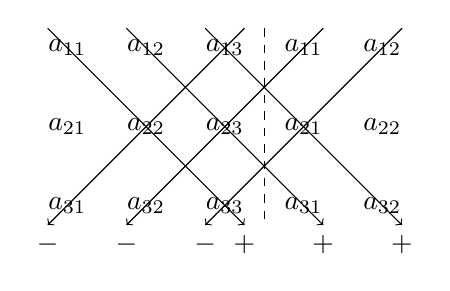
\begin{tikzpicture}
\draw[->] (-0.25,0.25) --(2.25,-2.25) node[anchor=north]{$+$};
\draw[->] (0.75,0.25) --(3.25,-2.25) node[anchor=north]{$+$};
\draw[->] (1.75,0.25) --(4.25,-2.25) node[anchor=north]{$+$};

\draw[->] (2.25,0.25) --(-0.25,-2.25) node[anchor=north]{$-$};
\draw[->] (3.25,0.25) --(0.75,-2.25) node[anchor=north]{$-$};
\draw[->] (4.25,0.25) --(1.75,-2.25) node[anchor=north]{$-$};
\draw (0,0) node {$a_{11}$};
\draw (1,0) node {$a_{12}$};
\draw (2,0) node {$a_{13}$};

\draw (0,-1) node {$a_{21}$};
\draw (1,-1) node {$a_{22}$};
\draw (2,-1) node {$a_{23}$};

\draw (0,-2) node {$a_{31}$};
\draw (1,-2) node {$a_{32}$};
\draw (2,-2) node {$a_{33}$};

\draw (3,0) node {$a_{11}$};
\draw (4,0) node {$a_{12}$};

\draw (3,-1) node {$a_{21}$};
\draw (4,-1) node {$a_{22}$};

\draw (3,-2) node {$a_{31}$};
\draw (4,-2) node {$a_{32}$};

\draw[dashed](2.5,0.25)--(2.5,-2.25);

\end{tikzpicture}
\end{center}
In this case the determinant is given by the product of the diagonals left to right, minus the product of the diagonals right to left. This is called the \textit{rule of Sarrus}. Note that \textit{rule of Sarrus} does not work for matrices with size greater than 3.\\

Most of the time, we use gaussian elimination to compute the determinant. We can use the cofactor formula mostly when $A$ has many zeroes. 

\section{Cramer's Rule}
\textit{Cramer's rule} is an explicit formula for the solution of a linear system of equations with \textit{as many equations as unknowns}, valid whenever the system has a \textit{unique} solution.\\
Let us consider the equation $$A\ul{x} = \ul{b}$$ 
where $A = \begin{pmatrix}
a_{11} & a_{12} & a_{13}\\
a_{21} & a_{22} & a_{23}\\
a_{31} & a_{32} & a_{33}\\
\end{pmatrix}$, $\ul{x} = \begin{pmatrix}
x_1\\
x_2\\
x_3
\end{pmatrix}$ and $\ul{b} = \begin{pmatrix}
b_1\\
b_2\\
b_3
\end{pmatrix}$\\ \\
So, our equation is
\[
\begin{pmatrix}
a_{11} & a_{12} & a_{13}\\
a_{21} & a_{22} & a_{23}\\
a_{31} & a_{32} & a_{33}\\
\end{pmatrix}\cdot \begin{pmatrix}
x_1\\
x_2\\
x_3
\end{pmatrix} = \begin{pmatrix}
b_1\\
b_2\\
b_3
\end{pmatrix}
\]
We can then substitute the first column of $A$ with $\ul{b}$, and we call this new matrix $B_1$:
\[
\begin{pmatrix}
a_{11} & a_{12} & a_{13}\\
a_{21} & a_{22} & a_{23}\\
a_{31} & a_{32} & a_{33}\\
\end{pmatrix}\cdot \begin{pmatrix}
x_1 & 0 & 0\\
x_2 & 1 & 0\\
x_3 & 0 & 1
\end{pmatrix} = \begin{pmatrix}
b_{1} & a_{12} & a_{13}\\
b_{2} & a_{22} & a_{23}\\
b_{3} & a_{32} & a_{33}\\
\end{pmatrix} = B_1
\]\\ \\
According to the properties of calculating the determinant of a matrix, we know that:
$$\det(A\cdot B) = \det(A)\cdot \det(B)$$
We can apply this rule to calculate the determinant of $$\begin{pmatrix}
a_{11} & a_{12} & a_{13}\\
a_{21} & a_{22} & a_{23}\\
a_{31} & a_{32} & a_{33}\\
\end{pmatrix}\cdot \begin{pmatrix}
x_1 & 0 & 0\\
x_2 & 1 & 0\\
x_3 & 0 & 1
\end{pmatrix}$$
So we have:
$$\det(A) \cdot \det\begin{pmatrix}
x_1 & 0 & 0\\
x_2 & 1 & 0\\
x_3 & 0 & 1
\end{pmatrix} = \det(B_1)$$
Note that $\begin{pmatrix}
x_1 & 0 & 0\\
x_2 & 1 & 0\\
x_3 & 0 & 1
\end{pmatrix}$ is a lower triangular matrix, thus its determinant is the product of the diagonal entries, thus its determinant is $x_1$:
\begin{align*}
\det(A)\cdot x_1 &= \det(B_1)\\
x_1 &=\frac{\det(B_1)}{\det(A)}
\end{align*}\\
Similarly, we can again substitute the second row of $A$ with $\ul{b}$ to form $B_2$:
\[
\begin{pmatrix}
a_{11} & a_{12} & a_{13}\\
a_{21} & a_{22} & a_{23}\\
a_{31} & a_{32} & a_{33}\\
\end{pmatrix}\cdot \begin{pmatrix}
1 & x_1 & 0\\
0 & x_2 & 0\\
0 & x_3 & 1
\end{pmatrix} = \begin{pmatrix}
a_{11} & b_{1} & a_{13}\\
a_{21} & b_{2} & a_{23}\\
a_{23} & b_{3} & a_{33}\\
\end{pmatrix} = B_2
\]

\begin{align*}
\det(A)\cdot x_2 &= \det(B_2)\\
x_2 &=\frac{\det(B_2)}{\det(A)}
\end{align*}\\
In general
\[
x_i = \frac{\det(B_i)}{\det(A)}, i=1,\dots,n
\]
where $B_i$ is $A$ with column $i$ replaced by $\ul{b}$, where $\det(A)\not=0$ (division by zero is not defined).

\begin{example}
Suppose we want to find the solutions to the following linear system of equations:
$$\begin{rightalignedcases}
3x+2y+4z=1\\
2x-y+z=0\\
x+2y+3z=1
\end{rightalignedcases}$$
We first create the matrix $A$ with the coefficients of the addends that are on the left side of the equals sign of each equation:
$$A=\begin{pmatrix}
3 & 2 & 4\\
2 & -1 & 1\\
1 & 2 & 3
\end{pmatrix}$$
and similarly we create the vector $\ul{b}$ using the numbers on the right side of the equals sign of each equation:
$$\ul{b}=\colvec{3}{1}{0}{1}$$
Now, we just need to find $B_1$, $B_2$ and $B_3$ using the process described above:
$$B_1 = \left(\begin{matrix}
1 & 2 & 4\\
0 & -1 & 1\\
1 & 2 & 3	
\end{matrix}\right)$$

$$B_2 = \left( \begin{matrix}
3 & 1 & 4\\
2 & 0 & 1\\
1 & 1 & 3
\end{matrix}\right)$$

$$B_3 = \left( \begin{matrix}
3 & 2 & 1\\
2 & -1 & 0\\
1 & 2 & 1
\end{matrix}\right)$$
Finally, we calculate the determinant of each $B_i$ (where $i = 1...3$), and we divide it by the determinant of $A$ (which must be different from $0$) to find respectively $x$, $y$ and $z$:

$$x = \frac{\abs{\begin{matrix}
1 & 2 & 4\\
0 & -1 & 1\\
1 & 2 & 3	
\end{matrix}
}}{\abs{\begin{matrix}
3 & 2 & 4\\
2 & -1 & 1\\
1 & 2 & 3	
\end{matrix}
}} = -\frac{1}{5}$$ 

$$y = \frac{\abs{\begin{matrix}
3 & 1 & 4\\
2 & 0 & 1\\
1 & 1 & 3
\end{matrix}
}}{\abs{\begin{matrix}
3 & 2 & 4\\
2 & -1 & 1\\
1 & 2 & 3	
\end{matrix}
}} = 0$$ 

$$z= \frac{\abs{\begin{matrix}
3 & 2 & 1\\
2 & -1 & 0\\
1 & 2 & 1
\end{matrix}
}}{\abs{\begin{matrix}
3 & 2 & 4\\
2 & -1 & 1\\
1 & 2 & 3	
\end{matrix}
}} = \frac{2}{5}
$$

\end{example}

\section{Inverse of a Matrix}
We can use Cramer's rule also to find the inverse of a matrix.\\ \\
We know that if $$AX = XA = I$$ then $X$ is called the inverse of $A$, also denoted as $A^{-1}$.\\ \\ So we have that:
$$\begin{pmatrix}
a_{11} & \dots & a_{13}\\
\vdots & {} & \vdots\\
a_{31} & \dots & a_{33}
\end{pmatrix} \cdot \begin{pmatrix}
x_{11} & \dots & x_{13}\\
\vdots & {} & \vdots\\
x_{31} & \dots & x_{33}
\end{pmatrix} = \begin{pmatrix}
1 & 0 & 0\\
0 & 1 & 0\\
0 & 0 & 1\\
\end{pmatrix}$$
which implies that:
$$\begin{pmatrix}
a_{11} & \dots & a_{13}\\
\vdots & {} & \vdots\\
a_{31} & \dots & a_{33}
\end{pmatrix}\cdot \colvec{3}{x_{11}}{x_{21}}{x_{31}} = \colvec{3}{1}{0}{0}$$
Now, we can apply the \textit{Cramer's rule} to find $x_{11}$, $x_{21}$ and $x_{31}$:
$$x_{11} = \frac{\abs{\begin{matrix}
1 & a_{12} & a_{13}\\
0 & a_{22} & a_{23}\\
0 & a_{32} & a_{33}\\
\end{matrix}
}}{\det(A)} = \frac{c_{11}}{\det(A)}$$

$$ x_{21} = \frac{c_{12}}{\det(A)}$$
$$x_{31} = \frac{c_{13}}{\det(A)}$$ \\
In general, element $ij$ of $A^{-1}$ can be computed as: 
$$\left( A^{-1}\right)_{ij} = \frac{c_{ji}}{\det(A)}$$
Note that it is really $c_{ji}$ and \textbf{not} $c_{ij}$!